% Tiefpass Amplitudengang (MINIMAL), lineare Achsen, tau = 10 ms
\begin{tikzpicture}[x=1mm,y=1mm] % gilt für tikz-coordinaten außerhalb der axis-environment
    \draw[draw=none] (-14,-12) rectangle (54,22); % Bildrahmen, Koordinatenbezug auf (0,0) des \begin{axis}...\end{axis} pgfplots, für
    \begin{axis}[
        xmode=linear,
        ymode=linear,
        ylabel={$A(\omega/\omega_g)$},
        xlabel={$\omega/\omega_g$},
        xlabel style={yshift=+0pt},
        ylabel style={yshift=-1pt},
        %ylabel style={at={(axis description cs:-0.09,1)}, rotate=-90,},
        %xlabel style={at={(axis description cs:1,-0.15)}},
        xmin=0, xmax=2,
        domain=0:5,
        ymin=-0.1, ymax=1.1,
        samples=61,
        width=6.5cm,
        height=3.5cm,
        xtick distance=0.5,
        xticklabels={,$0$,,1,,2},
        ytick distance=0.5,
        yticklabels={,$0$,,$1$},
        grid=both,
        extra tick style={grid=none,style={draw=none}},
        extra y ticks={0.7071},
        extra y tick labels={$\sfrac{1}{\sqrt{2}}$},
    ]
        % omega_g, Bereiche
        \addplot+[mark=none,draw=black,dashed] coordinates{(0,0.7071)(1,0.7071)};
        \addplot+[mark=none,draw=black,dashed] coordinates{(1,-0.1)(1,1.1)};
        \addplot+[mark=none,draw=none] coordinates{(0,0)(2,0)} 
            node[pos=0.25,anchor=south,black] {Durchlassber.}
            node[pos=0.75,anchor=south,black,yshift=-2pt] {Sperrbereich}; % yshift wegen Buchstabe "p"

        % plots
        \draw[thick,blue] (0,1) -- 
            (0.95,1.00) .. controls (1,1) .. (1.00,0.95) -- 
            (1.00,0.05) .. controls (1,0) .. (1.05,0.00) -- 
            (2,0); % ideal
        \addplot+[mark=none,very thick,red]   {1/(1+x^2)^0.5}; % real
        
        % plotlabel
        \addplot+[mark=none,draw=none] coordinates {(1,0.9)} node[anchor=west,blue] {ideal};
        \addplot+[mark=none,draw=none] coordinates {(1.6,0.7)} node[anchor=west,red] {real};
        %\addplot+[mark=none,draw=none, red] coordinates {(1.1,)} node[pos=0,pin=-90:$\frac{1}{\sqrt{2}}$] {};

    \end{axis}
\end{tikzpicture}